\section{Recall results for GCF ablation study}\label{app:recall-results-gcf-ablation}
This section contains the results for the experiment described in \autoref{subsec:gcf-ablation-study}.

\begin{figure}[]
    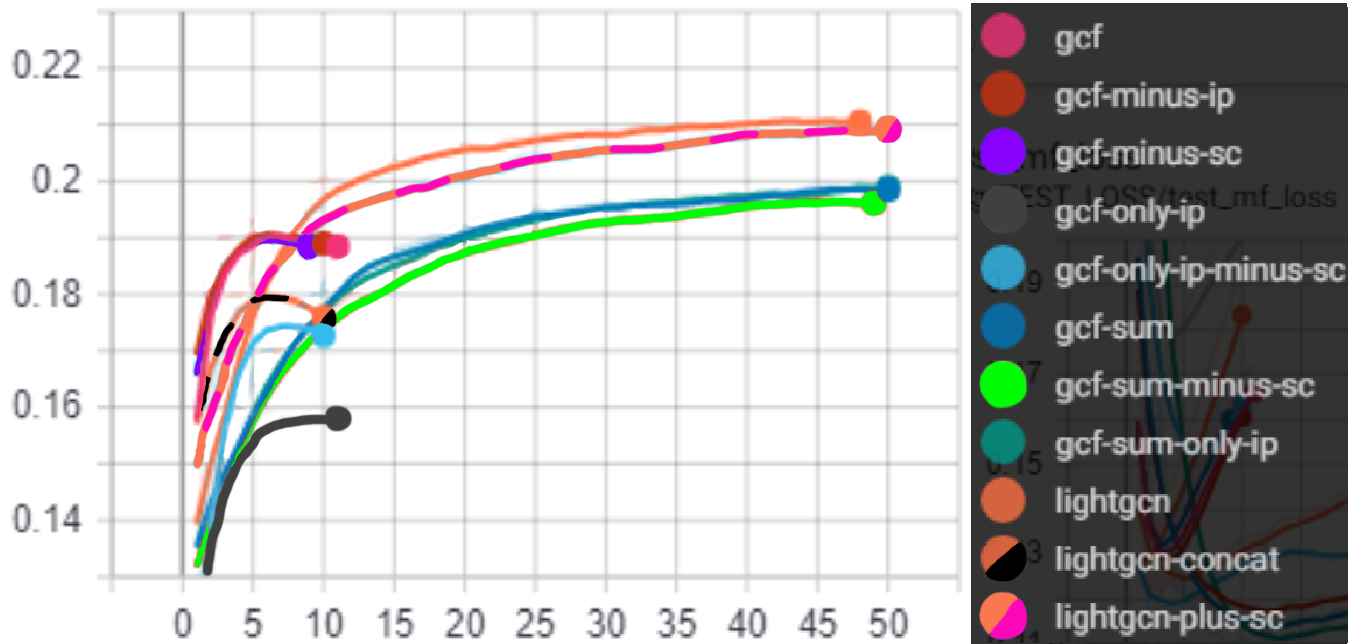
\includegraphics[width=\linewidth]{figures/gcf-all-recall.png}
    \caption{Recall@50 on the Yelp2020 dataset.}
    \label{fig:GCF-recall-ablation-study}
\end{figure}
\begin{figure}[]
    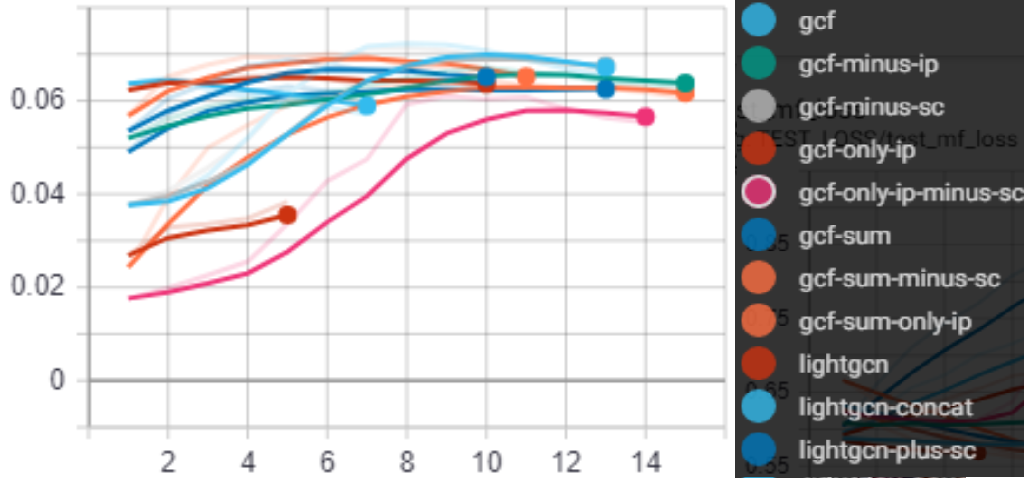
\includegraphics[width=\linewidth]{figures/amazon-cell-sport-gcf-all-recall.png}
    \caption{Recall@50 on the Amazon-Sport-Cell dataset.}
    \label{fig:GCF-recall-ablation-study-amazon-cell-sport}
\end{figure}
\begin{figure}[]
    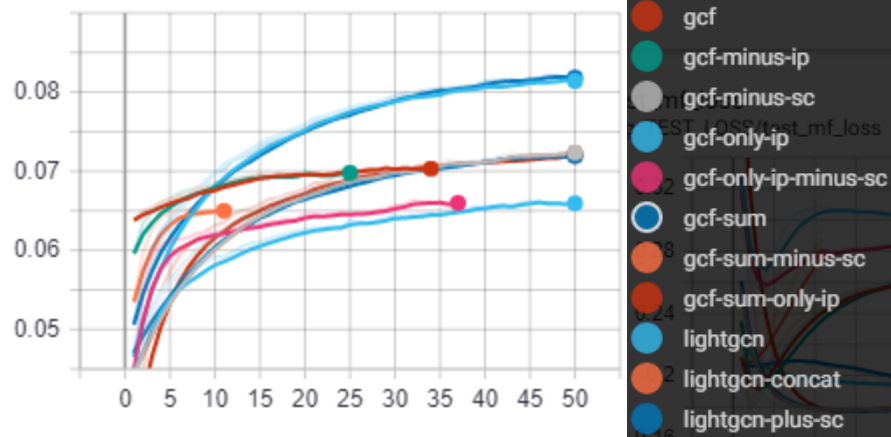
\includegraphics[width=\linewidth]{figures/amazon-book-gcf-all-recall.png}
    \caption{Recall@50 on the Amazon-Book dataset.}
    \label{fig:GCF-recall-ablation-study-amazon-book}
\end{figure}
\begin{figure}[]
    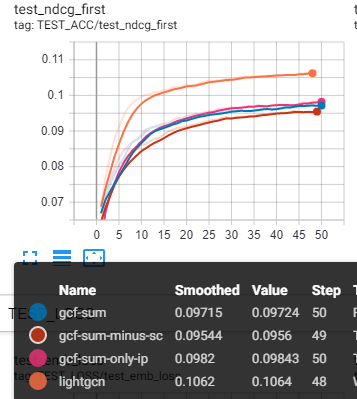
\includegraphics[width=\linewidth]{figures/gcf-sum-ndcg.png}
    \caption{NDCG@50 for the compared methods that utilize summation as layer combination on the Yelp2020 dataset.}
    \label{fig:GCF-sum-NDCG-ablation-study}
\end{figure}
\begin{figure}[]
    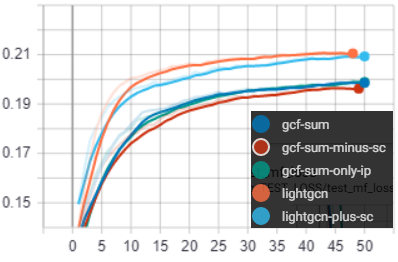
\includegraphics[width=\linewidth]{figures/gcf-sum-recall.png}
    \caption{Recall@50 on the compared methods that utilize summation as layer combination on the Yelp2020 dataset.}
    \label{fig:GCF-sum-recall-ablation-study}
\end{figure}
\begin{figure}[]
    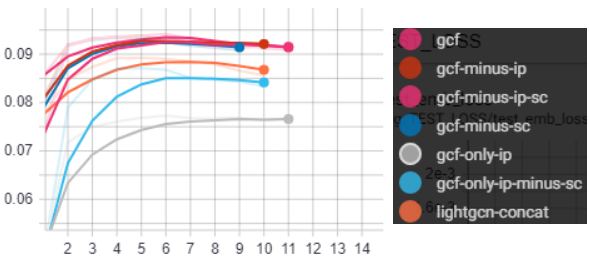
\includegraphics[width=\linewidth]{figures/gcf-ndcg-concat.png}
    \caption{NDCG@50 for the compared methods that utilize concatenation as layer combination on the Yelp2020 dataset.}
    \label{fig:GCF-NDCG-concat-ablation-study}
\end{figure}
\begin{figure}[]
    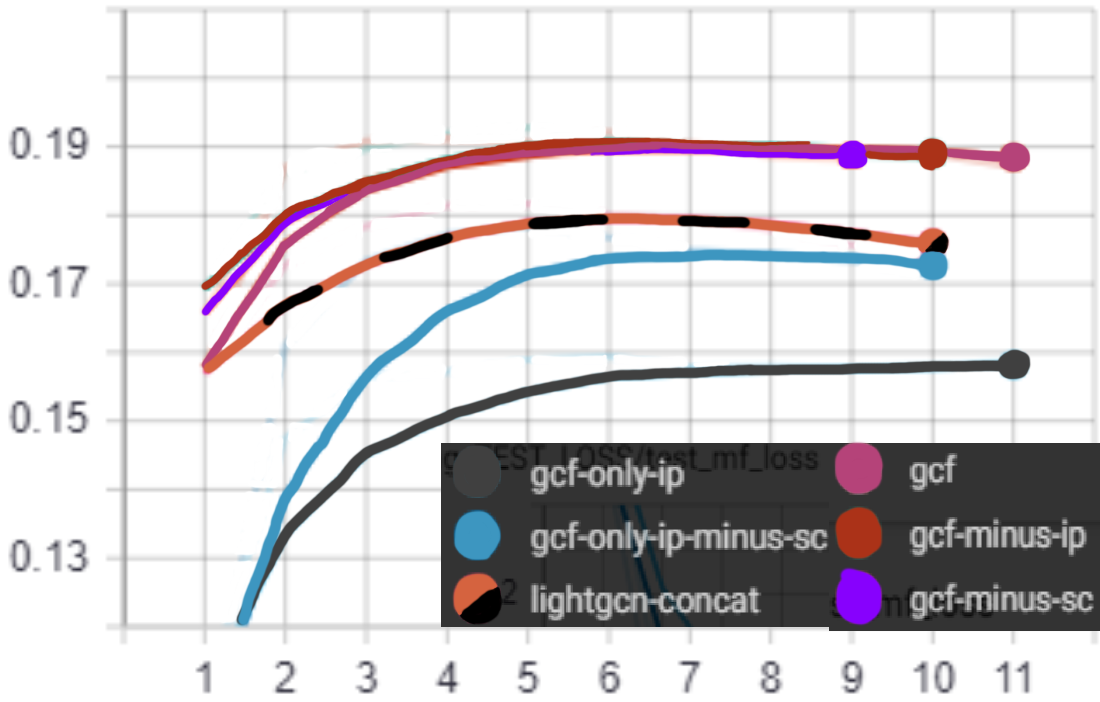
\includegraphics[width=\linewidth]{figures/gcf-concat-recall.png}
    \caption{Recall@50 for the compared methods that utilize concatenation as layer combination on the Yelp2020 dataset.}
    \label{fig:GCF-recall-concat-ablation-study}
\end{figure}
\begin{figure}[]
    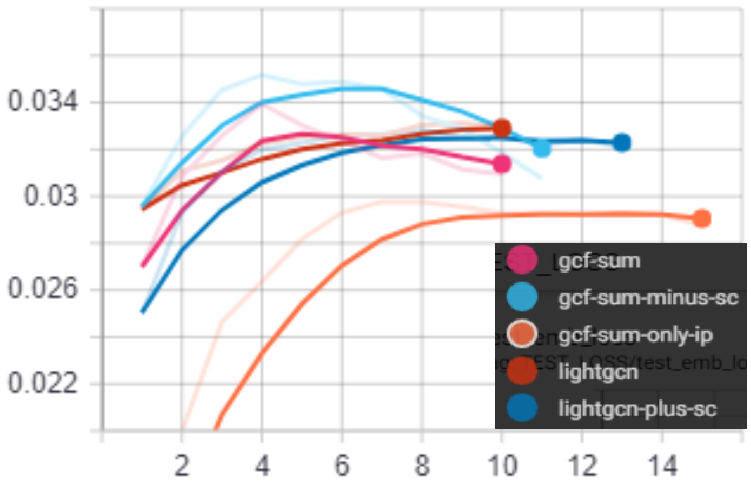
\includegraphics[width=\linewidth]{figures/amazon-cell-sport-gcf-sum-ndcg.png}
    \caption{NDCG@50 for the compared methods that utilize summation as layer combination on the Amazon-Cell-Sport dataset.}
    \label{fig:GCF-sum-NDCG-ablation-study-Amazon-Cell-Sport}
\end{figure}
\begin{figure}[]
    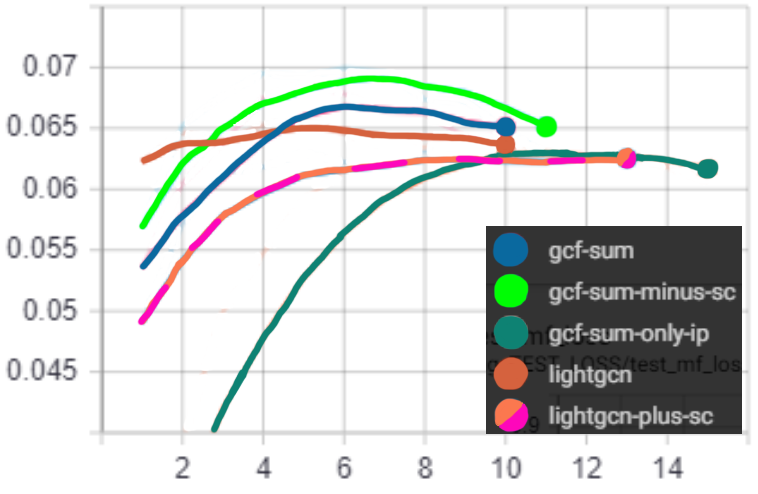
\includegraphics[width=\linewidth]{figures/amazon-cell-sport-gcf-sum-recall.png}
    \caption{Recall@50 on the compared methods that utilize summation as layer combination on the Amazon-Cell-Sport dataset.}
    \label{fig:GCF-sum-recall-ablation-study-Amazon-Cell-Sport}
\end{figure}
\begin{figure}[]
    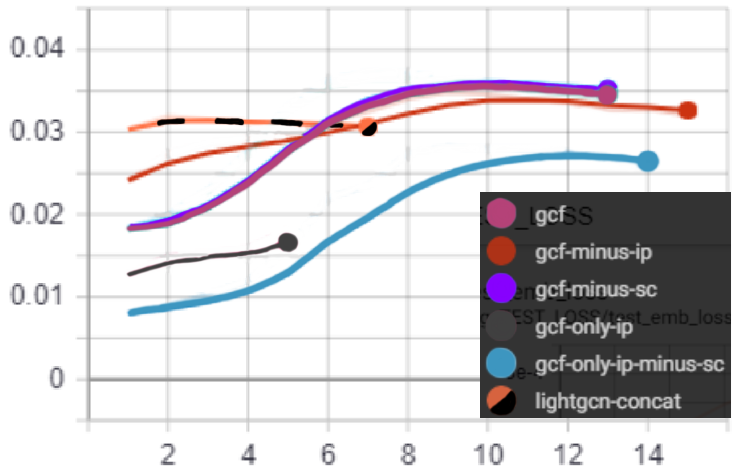
\includegraphics[width=\linewidth]{figures/amazon-cell-sport-gcf-ndcg.png}
    \caption{NDCG@50 for the compared methods that utilize concatenation as layer combination on the Amazon-Cell-Sport dataset.}
    \label{fig:GCF-NDCG-concat-ablation-study-Amazon-Cell-Sport}
\end{figure}
\begin{figure}[]
    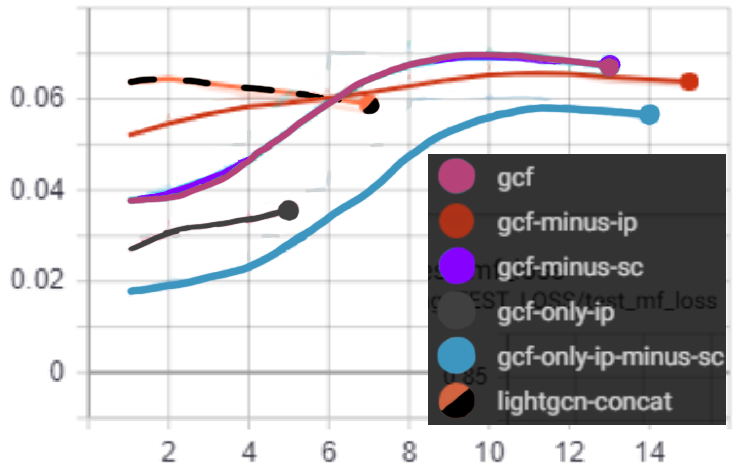
\includegraphics[width=\linewidth]{figures/amazon-cell-sport-gcf-recall.png}
    \caption{Recall@50 for the compared methods that utilize concatenation as layer combination on the Amazon-Cell-Sport dataset.}
    \label{fig:GCF-recall-concat-ablation-study-Amazon-Cell-Sport}
\end{figure}
\begin{figure}[]
    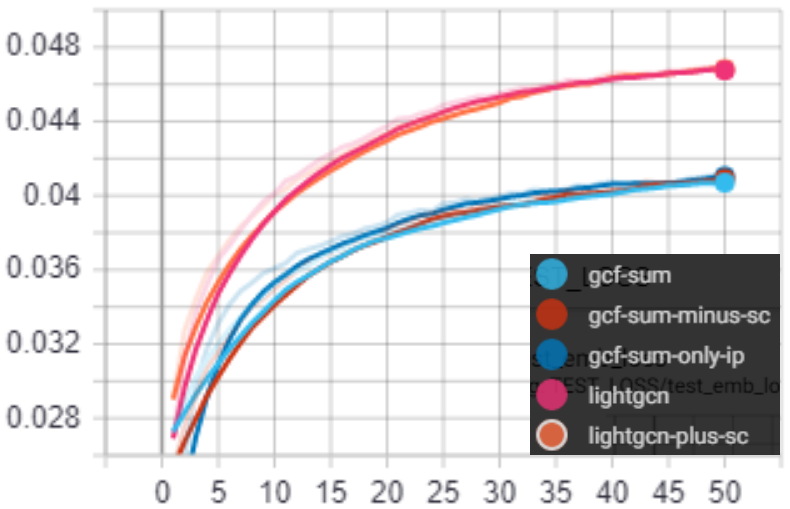
\includegraphics[width=\linewidth]{figures/amazon-book-gcf-sum-ndcg.png}
    \caption{NDCG@50 for the compared methods that utilize summation as layer combination on the Amazon-Book dataset.}
    \label{fig:GCF-sum-NDCG-Amazon-Book-ablation-study}
\end{figure}
\begin{figure}[]
    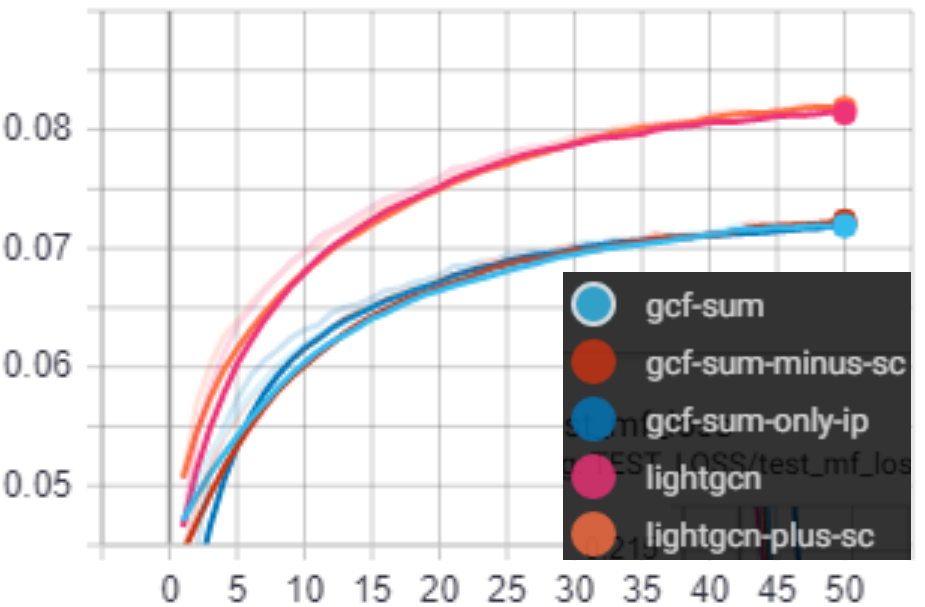
\includegraphics[width=\linewidth]{figures/amazon-book-gcf-sum-recall.png}
    \caption{Recall@50 on the compared methods that utilize summation as layer combination on the Amazon-Book dataset.}
    \label{fig:GCF-sum-recall-Amazon-Book-ablation-study}
\end{figure}
\begin{figure}[]
    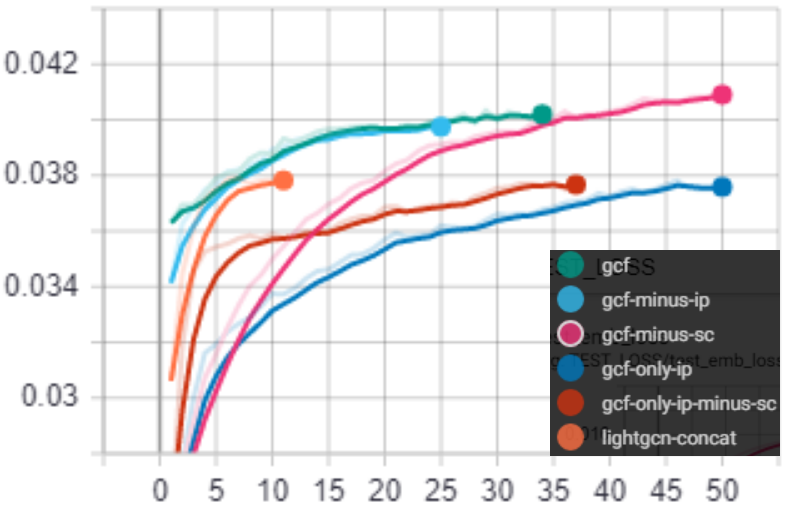
\includegraphics[width=\linewidth]{figures/amazon-book-gcf-concat-ndcg.png}
    \caption{NDCG@50 for the compared methods that utilize concatenation as layer combination on the Amazon-Book dataset.}
    \label{fig:GCF-NDCG-concat-Amazon-Book-ablation-study}
\end{figure}
\begin{figure}[]
    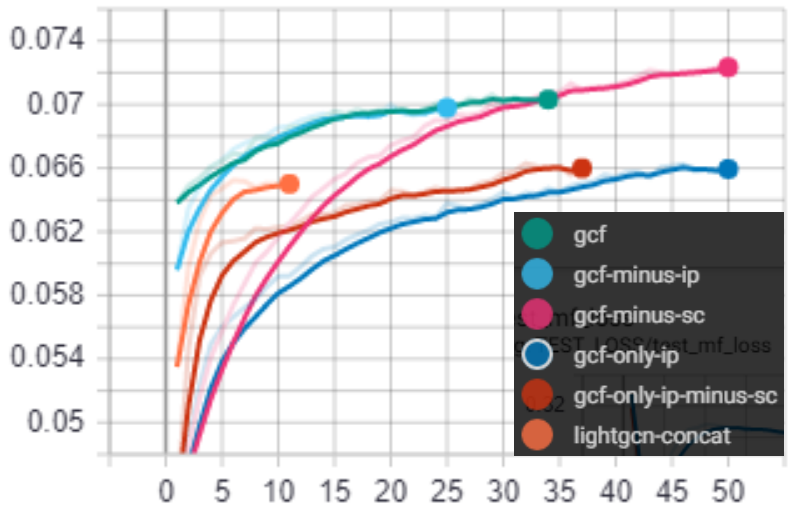
\includegraphics[width=\linewidth]{figures/amazon-book-gcf-concat-recall.png}
    \caption{Recall@50 for the compared methods that utilize concatenation as layer combination on the Amazon-Book dataset.}
    \label{fig:GCF-recall-concat-Amazon-Book-ablation-study}
\end{figure}